\documentclass[t,aspectratio=169,14pt]{beamer}  % [t], [c], или [b] --- вертикальное выравнивание на слайдах (верх, центр, низ)
%\documentclass[handout]{beamer} % Раздаточный материал (на слайдах всё сразу)
%\documentclass[t,aspectratio=169]{beamer} % Соотношение сторон

\usetheme{Madrid}
\usecolortheme{seahorse}

%%% Работа с русским языком
\usepackage{cmap}					% поиск в PDF
%\usepackage{mathtext} 				% русские буквы в формулах
\usepackage[T2A]{fontenc}			% кодировка
\usepackage[utf8]{inputenc}			% кодировка исходного текста
\usepackage[russian]{babel}	% локализация и переносы
\usefonttheme{serif} % default, serif, professionalfonts, structurebold, structureitalicserif,structuresmallcapsserif 

%%% Работа с картинками
\usepackage{graphicx}  % Для вставки рисунков
\graphicspath{{images}}  % папки с картинками
\setlength\fboxsep{3pt} % Отступ рамки \fbox{} от рисунка
\setlength\fboxrule{1pt} % Толщина линий рамки \fbox{}
%\usepackage{wrapfig} % Обтекание рисунков текстом
\setbeamertemplate{caption}{\raggedright\insertcaption\par}
%[numbered] % set captions with numbers
%%% Другие пакеты
\usepackage{lastpage} % Узнать, сколько всего страниц в документе.
\usepackage{soul} % Модификаторы начертания
\usepackage{csquotes} % Еще инструменты для ссылок
%\usepackage[style=authoryear,maxcitenames=2,backend=biber,sorting=nty]{biblatex}
\usepackage{multicol} % Несколько колонок
\usepackage{hyperref}
\hypersetup{				% Гиперссылки
	unicode=true,           % русские буквы в раздела PDF
	pdftitle={Запоминать Писание Наизусть},   % Заголовок
	pdfauthor={Библейская церковь Санкт-Петербурга},      % Автор
	pdfsubject={Тема},      % Тема
	pdfcreator={Создатель}, % Создатель
	pdfproducer={Производитель}, % Производитель
	pdfkeywords={keyword1} {key2} {key3}, % Ключевые слова
	colorlinks=false,       	% false: ссылки в рамках; true: цветные ссылки
	linkcolor=red,          % внутренние ссылки
	citecolor=black,        % на библиографию
	filecolor=magenta,      % на файлы
	urlcolor=cyan           % на URL
}

\def\hy#1{\parbox{\linewidth}{#1}} % hypenate text

%-------------------------------------------------------
\title{\textsc{\textbf{Запоминать Писание Наизусть}}}
\subtitle{Зачем и Как}
\author[Библейская Церковь СПб]{}

\titlegraphic{\vspace{-1.5cm}
\includegraphics[width=7cm]{bible-church-spb-logo}}
\date{}

% Change example block width
\addtobeamertemplate{block example begin}{%
    \setlength{\textwidth}{0.45\textwidth}
}{}

\usepackage{etoolbox}

\makeatletter
\patchcmd{\beamer@sectionintoc}{\vskip1.5em}{\vskip0.3em}{}{}
\patchcmd{\beamer@subsectionintoc}{\vskip1.5em}{\vskip0.5em}{}{}
\makeatother

\addtobeamertemplate{block begin}{\vfill}{}
\addtobeamertemplate{block end}{}{\vfill}

\begin{document}

\frame[plain]{\titlepage}	% Титульный слайд
%-------------------------------------------------------
\begin{frame}{Содержание}
	% \begin{multicols}{2}
    \tableofcontents[hideallsubsections]
	% \end{multicols}
\end{frame}
%-------------------------------------------------------
\section{Пять способов питания Божим Словом}
\begin{frame}
	\frametitle{\insertsection} 
	\framesubtitle{\insertsubsection}
	
	\begin{multicols}{2}
	\begin{enumerate}
		\item Слушать \pause
		\item Читать \pause
		\item Изучать \pause
		\item Запоминать \pause
		\item Размышлять и Применять
	\end{enumerate}
	\begin{figure}
		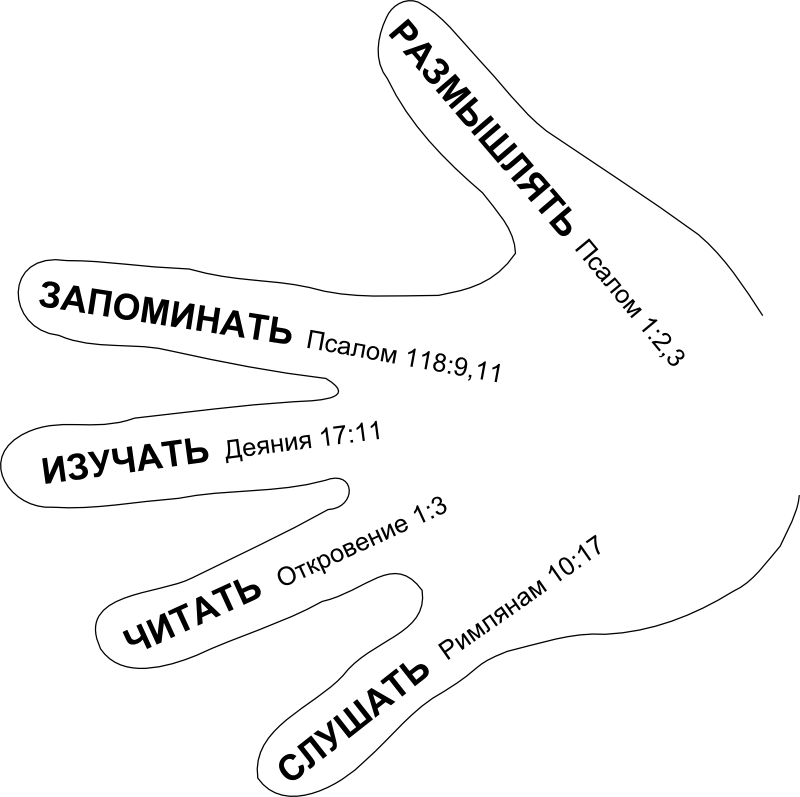
\includegraphics[height=0.6\textheight]{hand-word-ru-800}
		\caption{Иллюстрация <<Рука--Слово>>}
	\end{figure}	
	\end{multicols}
\end{frame}
%-------------------------------------------------------
\section{Заповеди}
% \subsection{Заповеди}
\begin{frame}
	\frametitle{\insertsection}

	\begin{block}{Второзаконие 6:6}
	И да будут слова сии, которые Я заповедую тебе сегодня, в сердце твоем. 
	\end{block}

\end{frame}  
%-------------------------------------------------------
\begin{frame}
	\frametitle{\insertsection}


	\begin{block}{Псалом 118:9,11}
	\hy{Как юноше содержать в~чистоте путь свой? --- Хранением себя по слову Твоему\ldots{} 
	\underline{В~сердце моем сокрыл я~слово Твое}, чтобы не грешить пред Тобою. }
	\end{block}	

\end{frame}  
%-------------------------------------------------------
\begin{frame}
	\frametitle{\insertsection}

	\begin{block}{Иисуса Навина 1:8}
		\hy{Да не отходит сия книга закона от уст твоих; но поучайся в~ней день и~ночь, дабы в~точности исполнять все, что в~ней написано: тогда ты будешь успешен в~путях твоих и~будешь поступать благоразумно.}
	\end{block}
\end{frame}  
%-------------------------------------------------------
\section{Пример Иисуса}
\begin{frame}
	\frametitle{\insertsection}

\begin{block}{Луки 4:4 --- Второзаконие 8:3}
\hy{Иисус сказал ему в ответ: \underline{написано}, что не хлебом одним будет жить человек, но всяким словом Божиим. }
\end{block}

\begin{block}{Луки 4:8 --- Второзаконие 6:13}
	\hy{отойди от Меня, сатана; \underline{написано}: Господу Богу твоему поклоняйся, и~Ему одному служи. }
\end{block}

\begin{block}{Луки 4:12 --- Второзаконие 6:16}
Иисус сказал ему в ответ: \underline{сказано}: не искушай Господа Бога твоего. 
\end{block}

\end{frame}    
%-------------------------------------------------------
\section{Принципы запоминания}
\begin{frame}
	\frametitle{\insertsection}
	\framesubtitle{\insertsubsection}
	
	\begin{enumerate}[<+->]
		\item Дословно
        \item Записывайте и проговаривайте вслух
        \item Отмечайте
        \item Повторение
        \item Тематическая система
        \item Ссылки
    \end{enumerate}

	\begin{block}{}
		\only<1>{
			\begin{enumerate}
				\item Дословно запомненный стих легче цитировать. 
				\item Вы цитируете Божье Слово, а не вашу его интерпретацию.
			\end{enumerate}}		
        \only<2>{Подключайте механическую, зрительную и слуховую память.}

        \only<3>{Отмечайте в~тексте повторения, противопоставления, ритм, списки и проч.}

        \only<4>{\hy{Повторение~--- секрет прочного запоминания.
		С~каждым разом на повторение потребуется меньше времени и усилий. Повторение~--- ключ к тому, чтобы не~растерять запомненное.}}

		\only<5>{\hy{Запоминать стих вместе с~темой. Вам будут доступны многие стихи, связанные с~этой темой. Например, \textbf{<<Супружество>>:}
		Бытие~2:24; Ефесянам~5:25,28; Евреям~13:8; 1~Петра 3:7; Иеремия~32:39.}}

		\only<6>{\hy{В начале стиха и в~конце запоминайте ссылку стиха/отрывка. }}
    \end{block}
\end{frame}
%-------------------------------------------------------
\section{Тематическая Система Запоминания}
\begin{frame}[c]
	\frametitle{\insertsection}
	\framesubtitle{\insertsubsection}
	\begin{figure}
		\begin{flushright}
		\vspace{-1.8cm}
		
\includegraphics[height=1cm]{navs-logo}

	\end{flushright}
		\end{figure}
		\vspace{0.4cm}
	\hy{Это тщательно отобранные и~сгруппированные по темам 60~ключевых библейских стихов.
	Некоторые темы:}
	\vspace{-6pt}

	\begin{itemize}
		\item Слово Божье
		\item Молитва 
		\item Господство Христа
		\item Христос в центре
		\item Свидетельство
		\item Общение
		\item Растите в честности
		\item Растите в вере
	\end{itemize}		
\end{frame}
%-------------------------------------------------------
%\section{Инструменты}
\section{Карточки}
\begin{frame}[c]
	\frametitle{\insertsection}
	\framesubtitle{\insertsubsection}
	Пример карточек на плотной бумаге
	 \begin{multicols*}{2}
		\begin{figure}
			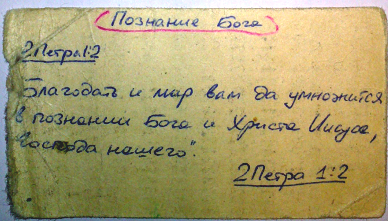
\includegraphics[height=0.4\textheight]{card-2Pe_1.2}
			% \caption{}
		\end{figure}
		\begin{figure}
			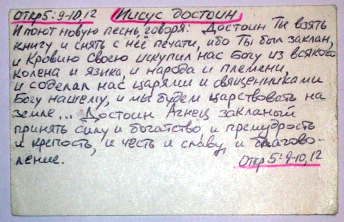
\includegraphics[height=0.4\textheight]{card-Re}
			% \caption{}
		\end{figure}	
	 \end{multicols*}
\end{frame}
%-------------------------------------------------------
\section{Приложение <<Помни Меня>>}
\begin{frame}[c]
	\frametitle{\insertsection}
%	\framesubtitle{\insertsubsection}
	\begin{figure}
		\begin{flushright}
		\vspace{-1.5cm}
		
\includegraphics[width=1cm]{remember-me-logo}
	\end{flushright}
		\end{figure}
		% \vspace{-0.2cm}

	 \begin{multicols}{2}
		Множество режимов разучивания % (словесные головоломки, заполнение пробелов, написание стихов)
		\begin{itemize}

			% \item Игры со случайными вопросами
			\item Карточки с разнесенными повторениями
			% \item Прослушивание или запись стихов
			% \item Извлечение библейских отрывков из онлайновых Библий
			\item Коллекции стихов
			% \item Синхронизация нескольких устройств
			% \item Многочисленные переводы Библии
			\item Гибкая маркировка и фильтры
			\item \textbf{www.remem.me}
			\item iOS, Android, Web
		\end{itemize}
		% \columnbreak
		\begin{center}
			\begin{figure}
			
			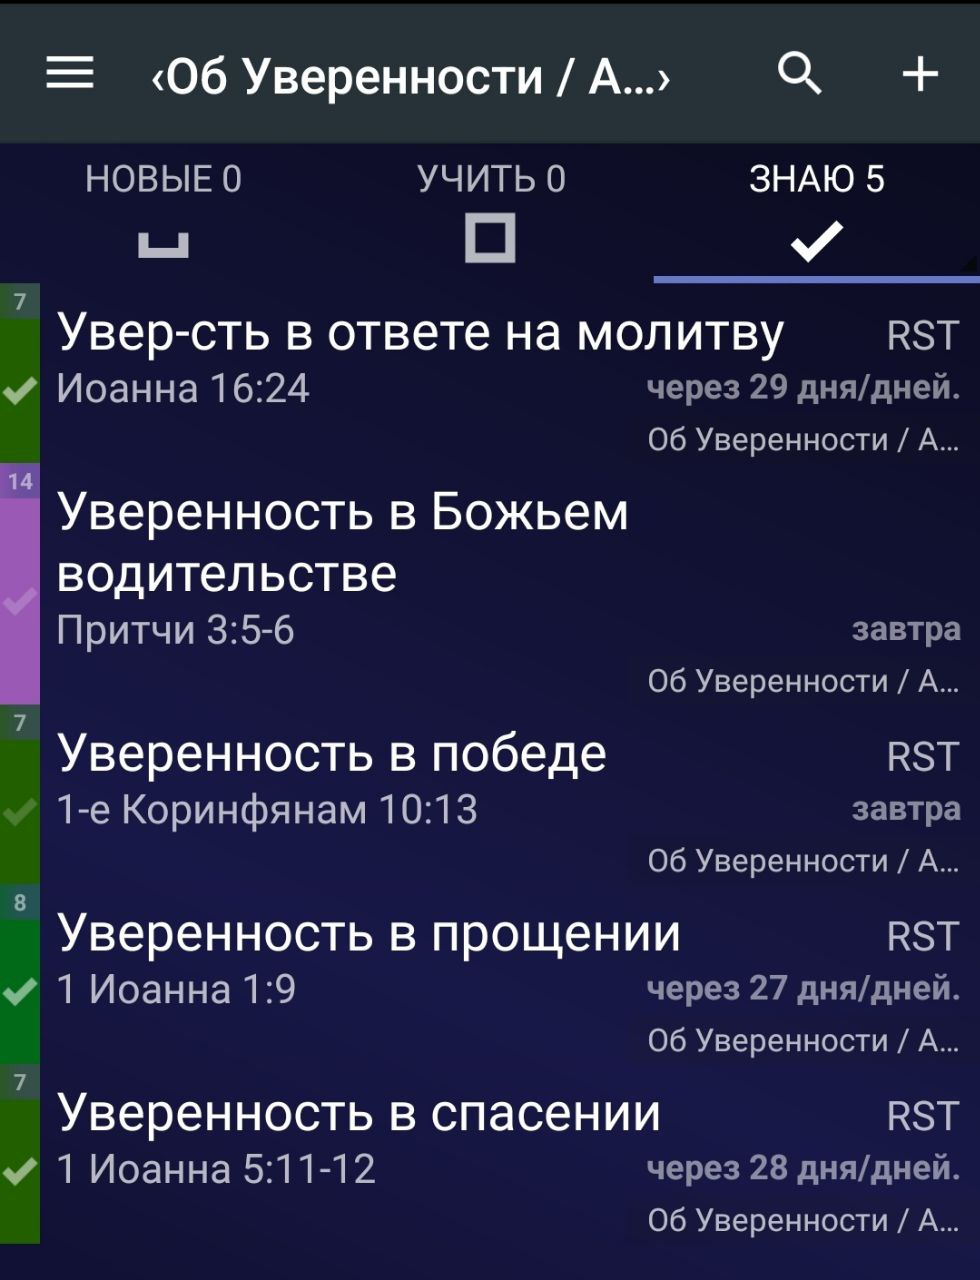
\includegraphics[height=0.8\textheight]{remember-me-lists}
			% \caption{Выбор слова}
			\end{figure}		
		\end{center}
	 \end{multicols}
\end{frame}
%-------------------------------------------------------
\begin{frame}[c]
	\frametitle{\insertsection}
%	\framesubtitle{\insertsubsection}
	\begin{figure}
		\begin{flushright}
		\vspace{-1.5cm}
		
\includegraphics[width=1cm]{remember-me-logo}
	\end{flushright}
		\end{figure}

	Режимы разучивания:
	 \begin{multicols}{2}
		\begin{center}
			\begin{figure}
			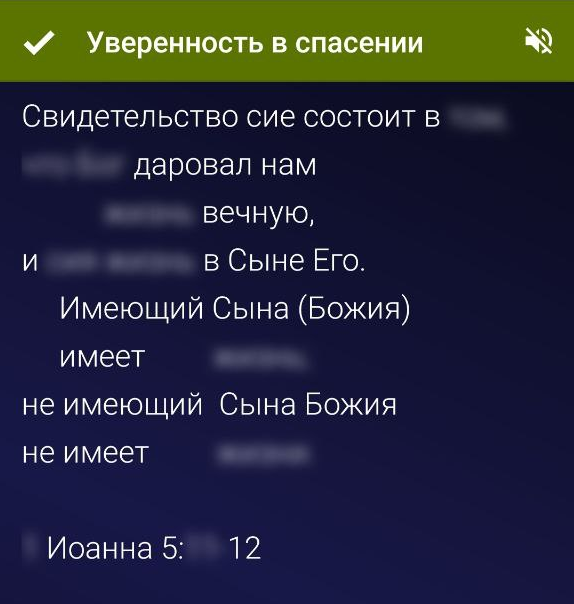
\includegraphics[height=0.55\textheight]{remember-me-card-hide}
			\caption{Скрытие слов}
			\end{figure}
			\begin{figure}
			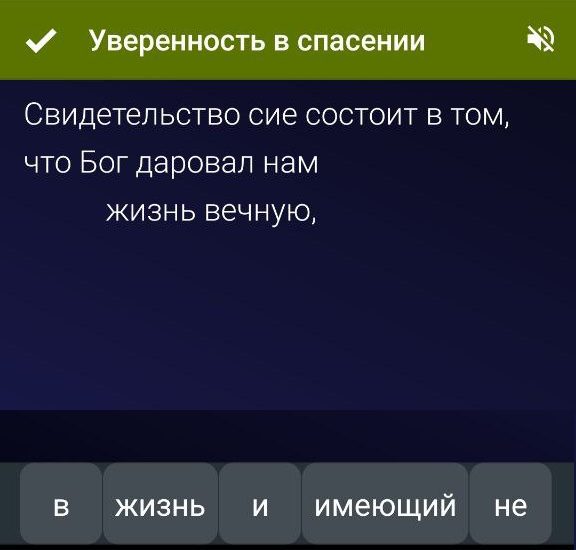
\includegraphics[height=0.55\textheight]{remember-me-card-pick}
			\caption{Выбор слова}
			\end{figure}		
		\end{center}
	 \end{multicols}
\end{frame}
%-------------------------------------------------------
\begin{frame}[c]
	\frametitle{\insertsection}
%	\framesubtitle{\insertsubsection}
	\begin{figure}
		\begin{flushright}
		\vspace{-1.5cm}
		
\includegraphics[width=1cm]{remember-me-logo}
	\end{flushright}
		\end{figure}

	Режимы разучивания:
	 \begin{multicols}{2}
		\begin{center}
			\begin{figure}
				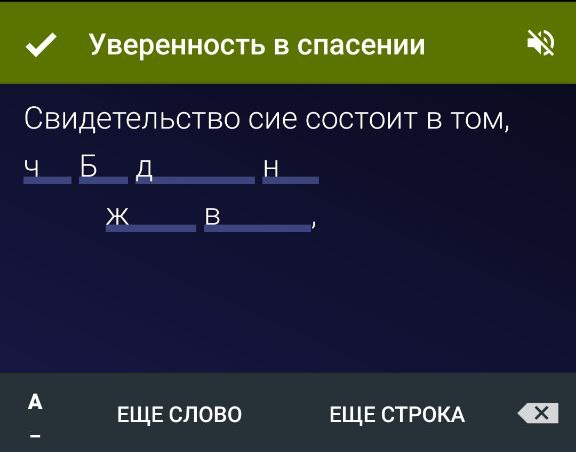
\includegraphics[height=0.55\textheight]{remember-me-card-hide-letters-underscores}
				\caption{Первые буквы слов}
				\end{figure}		
			\end{center}			
			\begin{figure}
			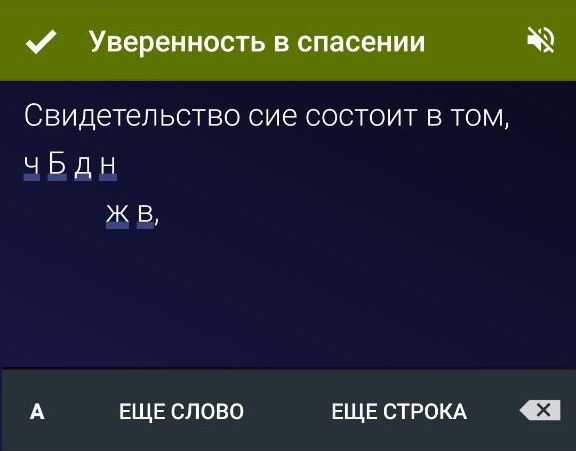
\includegraphics[height=0.55\textheight]{remember-me-card-hide-letter}
			\caption{Только первые буквы слов}
			\end{figure}

	 \end{multicols}
\end{frame}
%-------------------------------------------------------
\begin{frame}[c]
	\frametitle{\insertsection}
%	\framesubtitle{\insertsubsection}
	\begin{figure}
		\begin{flushright}
		\vspace{-1.5cm}
		
\includegraphics[width=1cm]{remember-me-logo}
	\end{flushright}
		\end{figure}

	Режимы разучивания:
	 \begin{multicols}{2}
		\begin{center}
			\begin{figure}
			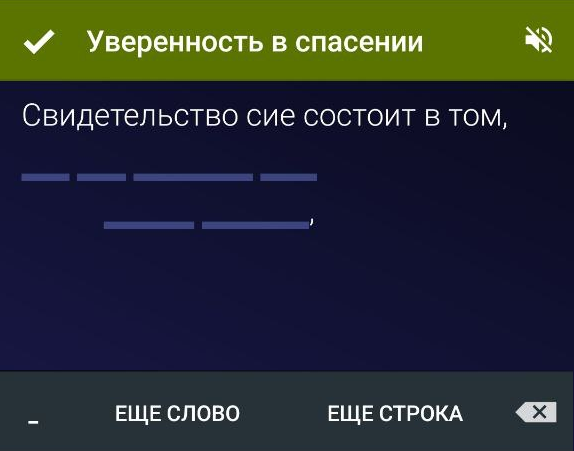
\includegraphics[height=0.55\textheight]{remember-me-card-hide-underscores}
			\caption{Контуры слов}
			\end{figure}
			\begin{figure}
			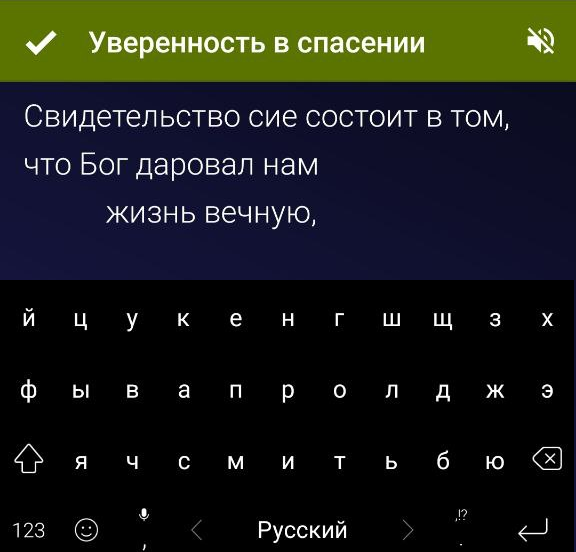
\includegraphics[height=0.55\textheight]{remember-me-card-type}
			\caption{Печать первой буквы}
			\end{figure}		
		\end{center}
	 \end{multicols}
\end{frame}
%-------------------------------------------------------
\section{Отзывы запоминающих Писание}
\begin{frame}[c]
	\frametitle{\insertsection}
	\framesubtitle{\insertsubsection}

	\begin{block}{Константин}
		\hy{Чаще всего слово приходит в виде вспоминающихся стихов в~конкретных, совершенно разных ситуациях. Когда сложно, они подсказывают направление. Если соглашаешься с~ними имеешь плод.}
	\end{block}
	
\end{frame}
%-------------------------------------------------------
\begin{frame}[c]
	\frametitle{\insertsection}
	\framesubtitle{\insertsubsection}

	\begin{block}{Ильдар}
		\hy{Сейчас трудное финансовое время. Стихи дают надежду и~утешение. Постоянно вспоминаю Филиппийцам 4:19. Приходят мысли разные депрессивные. Но вспоминаю стихи, и~мир приходит в~сердце и~энергия для дальнейших действий.}
		
		\vspace{6pt}
		
		\hy{<<Я был молод и состарился, и не видал праведника оставленным и~потомков его просящими хлеба>>. Псалом 36:25.}
	\end{block}
\end{frame}
%-------------------------------------------------------
\begin{frame}[c]
	\frametitle{\insertsection}
	\framesubtitle{\insertsubsection}

	\begin{block}{Максим}
		\hy{Я в юности выучил нагорную проповедь. Не поверишь от какого количества глупостей она меня удержала.}
	\end{block}
	\begin{block}{Яна}
	\hy{Я очень благодарна подруге, которая в своё время научила меня заучивать стихи и вместе со мной их учила на русском, и мы их обсуждали.}
	\end{block}
\end{frame}%-------------------------------------------------------
\begin{frame}[c]
	\frametitle{\insertsection}
	\framesubtitle{\insertsubsection}

	\begin{block}{Михаил}
		\hy{\ldots был момент, когда Дух Святой напомнил место Писания буквально за секунду до осознанного греха, что я намеревался сделать, зная, что это грех\ldots И я не сделал.}

		\vspace{6pt}

		\hy{Когда жене было трудно и она пребывала несколько лет в~депрессивном состоянии, я просто по кругу провозглашал все места, что знал.}
	\end{block}

\end{frame}
%-------------------------------------------------------
\section{Применение}
\subsection{Пять отрывков об уверенности}
\begin{frame}[c]
	\frametitle{\insertsection}
	\framesubtitle{\insertsubsection}
	\setbeamercolor{block title}{use=structure,fg=black,bg=purple!75!black}
	\setbeamercolor{block body}{use=structure,fg=white,bg=white!20!white}
	\begin{multicols}{2}
	\begin{exampleblock}{Уверенность в спасении}\setlength{\textwidth}{0.4\textwidth}
		1 Иоанна 5:11-12
	\end{exampleblock}
	\begin{exampleblock}{Уверенность в прощении}
		1 Иоанна 1:9
	\end{exampleblock}
	\begin{exampleblock}{Ув. в Божьем водительстве}
		Притчи 3:5-6
	\end{exampleblock}	
	\begin{exampleblock}{Ув. в ответе на молитву}
		Иоанна 16:24
	\end{exampleblock}	
	\begin{exampleblock}{Ув. в победе над грехом}
		1 Коринфянам 10:13
	\end{exampleblock}

	\end{multicols}		
\end{frame}
%-------------------------------------------------------
\subsection{Практика}
\begin{frame}[c]
	\frametitle{\insertsection}
	\framesubtitle{\insertsubsection}
	\begin{center}

  \begin{block}{Уверенность в спасении}
	1 Иоанна 5:11-12	 
	 \vspace{6pt}

	 Свидетельство сие состоит в~том, \newline
	 что Бог даровал нам жизнь вечную, \newline
	 и~сия жизнь — в~Сыне Его. %\newline
	 \vspace{5pt}

	 Имеющий\hspace{1cm} Сына [Божия] \hspace{0.9cm} имеет жизнь; \newline
	 не имеющий\hspace{0.5cm} Сына Божия \hspace{0.5cm} не имеет жизни.
	 \begin{flushright}
		1 Иоанна 5:11-12
	\end{flushright}
\end{block}
\end{center}
\end{frame}
%-------------------------------------------------------
\begin{frame}[c]
	%\frametitle{\insertsection}
	%\framesubtitle{\insertsubsection}
\begin{center}
	\LARGE www.remem.me

	\LARGE github.com/kdorichev/tms	

	\LARGE @kdorichev
\end{center}
\end{frame}

\end{document}